\documentclass[10pt]{article}
\usepackage{graphicx}
\usepackage[margin=1.5cm]{geometry}
\usepackage{amsmath}
\def\brcurs{{\mbox{$\resizebox{.16in}{.08in}{
\includegraphics{BoldR}}$}}}
\def\rcurs{{\mbox{$\resizebox{.16in}{.08in}{
\includegraphics{ScriptR}}$}}}

\begin{document}
\twocolumn

\title{Thursday Warm-up: Magnetic Fields and Work, Continuity Equation}
\author{Prof. Jordan C. Hanson}

\maketitle

\section{Memory Bank}

\begin{itemize}
\item \textbf{Lorentz force} on a constant current $I$ of length $\mathbf{L}$:
\begin{equation}
\mathbf{F} = I\mathbf{L} \times \mathbf{B}
\end{equation}
\item \textbf{Mechanical work}:
\begin{equation}
W = \int \mathbf{F} \cdot d\mathbf{l}
\end{equation}
\item \textbf{Continuity equation}:
\begin{equation}
\nabla \cdot \mathbf{J} = - \frac{\partial \rho}{\partial t}
\end{equation}
\end{itemize}

\begin{figure}
\centering
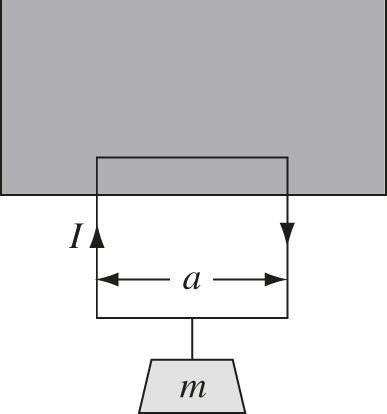
\includegraphics[width=0.2\textwidth]{figures/5_9.jpg} \hspace{0.5cm}
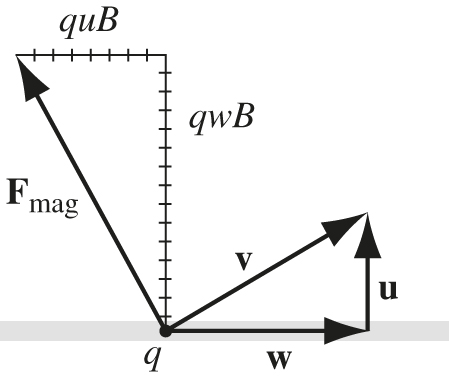
\includegraphics[width=0.25\textwidth]{figures/5_10.jpg}
\caption{\label{fig:1} (Left) A loop of wire passes through a region with $\mathbf{B}$ into the page, supporting a mass $m$.  (Right) The velocity components of the charge once the loop begins to move.}
\end{figure}

\section{Lorentz Force}

\begin{enumerate}
\item Using the definitions in the Memory Bank, prove that magnetic fields do no work. \\ \vspace{2cm}
\item A rectangular loop of wire, supporting a mass $m$, hangs vertically with one end in a uniform magnetic field $\mathbf{B}$, which points into the page in the shaded region of Fig. \ref{fig:1} (left).  What current $I$ would exactly balance the gravitational force downward? \\ \vspace{1cm}
\item If the current is \textit{increased} from the value that balances the weight, the mass \textit{rises.}\footnote{Students in PHYS180 did this experiment!  It's cool to watch.}  If the mass rises a distance $h$, work is being done against gravity.  Write down the product of the Lorentz force and $h$. \\ \vspace{1cm}
\item Suppose the loop rises with constant velocity $\mathbf{u} = u\mathbf{\hat{y}}$, and the current is $I = \lambda w\hat{\mathbf{x}}$.  (a) Show that the actual velocity of charge in the wire is $\mathbf{v} = \mathbf{u} + \mathbf{w}$.  (b) Derive the components of the net force on the charge $q$. \\ \vspace{2cm}
\item Let the total charge on the line segment $a$ be $q = \lambda a$.  (a) Show that the vertical and horizontal components of the Lorentz force in Fig. \ref{fig:1} (right) are $\lambda a w B$, and $\lambda a u B$, respectively. (b) What work must be done against the horizontal force in a time $dt$ to keep the current constant?  That is, evaluate:
\begin{equation}
W = \int F_{\rm horiz} dx = \int F_{\rm horiz} w dt
\end{equation}
Show this work is equal to the work required to lift the mass.
\end{enumerate}

\begin{figure}
\centering
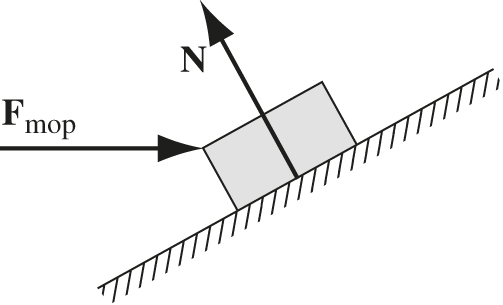
\includegraphics[width=0.35\textwidth]{figures/5_11.jpg}
\caption{\label{fig:2} Applied force, normal force, on an incline.}
\end{figure}

\end{document}
